%!TEX root = ../Thesis.tex
\chapter{Methodology}

\begin{figure}[ht]
    \hspace{-1.5cm}\centering
        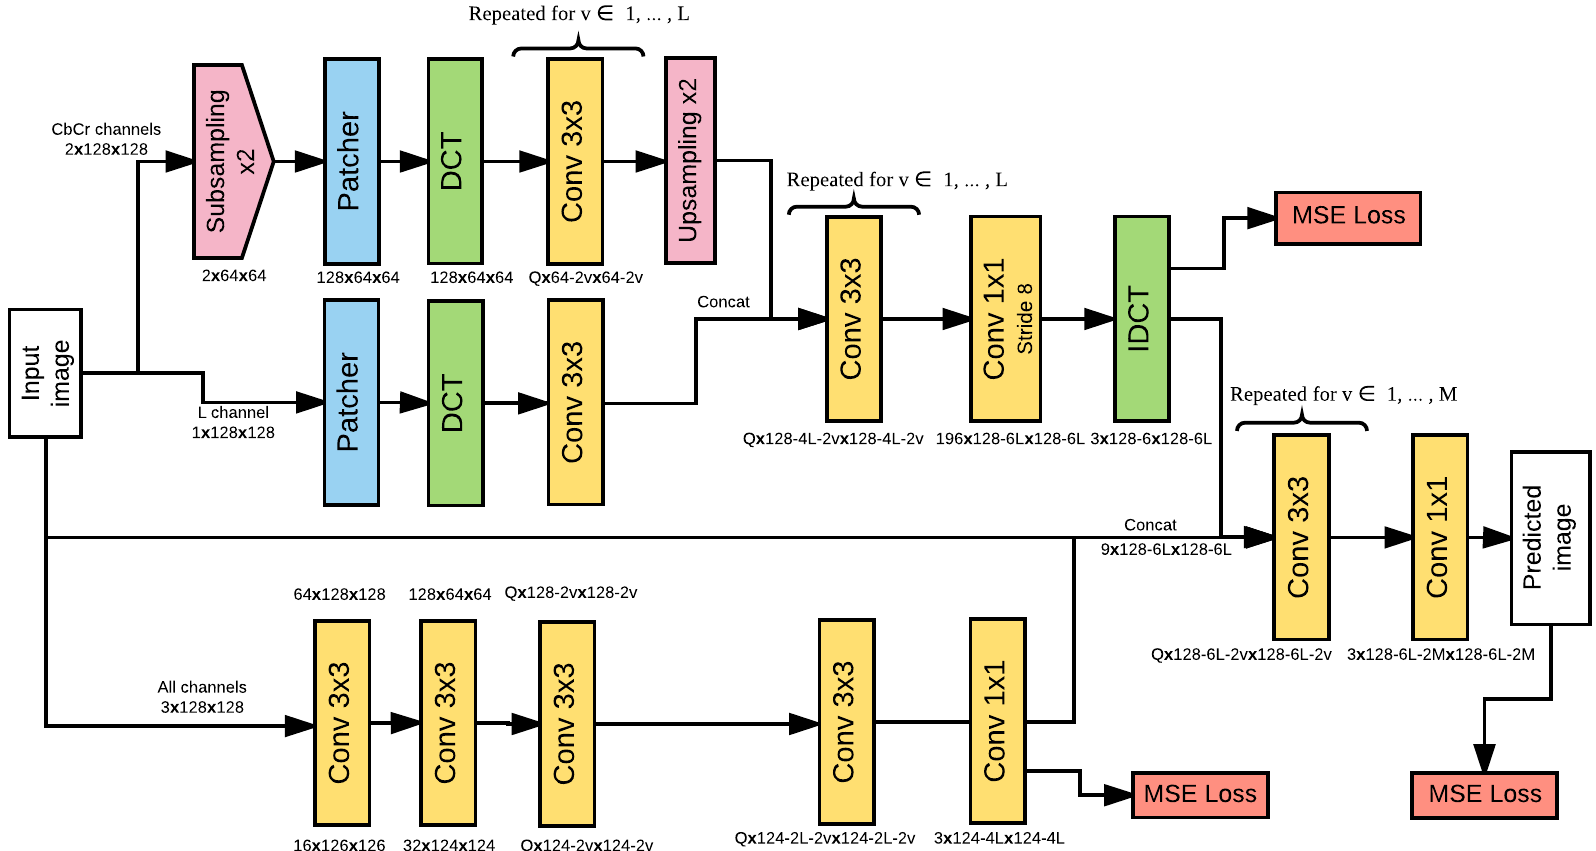
\includegraphics[width=1.1\textwidth]{../graphics/architecture.png}
    \caption[Short caption to special figure]{\textit{DDC-Net:} Proposed architecture which can exploit additional redundancies due to subsampling of the chroma components in JPEG compression. Every convolution layer is implicitly followed by a ReLu activation function.}
    \label{fig_archy}
\end{figure}


\subsection{DCT domain branch}
The first part of the DCT domain part of the network starts by splitting the Y (luma) component from the CbCr (chroma) components. The chroma component branch first features a downsampling of two in both x and y dimensions, this is done to match the 8$\times$8 coding blocks used in JPEG. Then in both the Y and the CbCr branch $L$ convolution layers with a $Q$ 3$\times$3 filters are stacked designed to exploit the redunancies present in the neighboring 8$\times$8 JPEG coding blocks. 

Prior to merging these two streams, the chroma component branch's feature maps are upscaled by a factor of two to match the luma branch spatially. This is followed by another series of $L$ convolutions. The main idea is that the chroma branch's pixels describe a 16x16 area, whereas in the luma branch this is a finer 8x8 pixels, fusing the information of both may improve both.

\section{Data Augmentation}
Artificially increasing the amount of data by adding variations of the original data can help train a model that generalizes well. Augmentation consists of applying (random) pertubations to the samples in ways that do not change the targets of these samples. For the problem of JPEG compression artifact removal we can simply determine the new targets as long as we perform these augmentations prior to generating the compressed version. 

Expanding the dataset through augmentation has a regularizing effect which helps prevent overfitting. Especially effective are augmentations that are also realistic examples of real world data. As such, we perform the following augmentation methods which we believe yield realistic new samples:

\begin{itemize}

\item \textbf{Flips}
The images are randomly mirrored in the X and/or Y direction, both with a 0.5 probability. 

\item \textbf{Rotations}
The images are randomly rotated 0, 90, 180, or 270 degrees with equal probability.

\item \textbf{Zooming}
The images are randomly magnified by a factor between 0.9 and 1.1 with uniform probability.

\item \textbf{HSV jittering}
HSV is a colorspace that represents a color image in three channels; a \emph{hue} (color), \emph{saturation} (vibrance) and a \emph{value} (brightness) channel. We randomly jitter the hue, saturation and vibrance of an image by multiplying it with a random value between -1.075 and 1.075. The values of all pixels are then clipped between 0 and 1.

\end{itemize}


\section{Implementation Details}
All methods were implemented using the publicy available PyTorch library for tensor computation and deep neural networks, which saw its beta release in January 2017. This library allows for GPU acceleration with CUDA and cuDNN primitives. All models were trained on a system with 16GB of RAM, an Intel i5-4670K at 3.6GHz, and an Nvidia Gefore GTX1080 graphics card. 

